For fiducial cross section measurements, we perform a maximum likelihood fit of the signal and background parameterisations to the observed $m_{4\ell}$ mass distribution and directly extract the parameter of interest ($\sigma{}_{fid}$). Definition of the likelihood function and the procedrue is explained in Section \ref{sec:StatProcedure}.

%The purpose is to extract integrated and differential fiducial cross sections after corrections of detector effects, resolution and systematic biases. To
%achieve
%this target, the corrections are extracted by using simulated samples and then encoded in the parametrization of $m_{4\ell}$ spectra at the
%reconstruction level. Then we directly extract the parameter of interest ($\sigma{}_{fid}$) by performing the maximum likelihood fit of background and
%signal
%parametrization to the observed $m_{4\ell}$ distribution.
%All the systematic uncertainties in the measurements are encoded as nuisance parameters, which are profited properly in fit procedure. In order to obtain results, we used asymptotic approach~\cite{Cowan:2010js} with test statistics that is based on profile likelihood ratio~\cite{LHC-HCG}. 
%Maximization of  likelihood is performed by fitting simultaneously, in each bin, the signal cross section at the fiducial level with all reconstruction bins and all three final states.
%The procedure applied for $\Hllll$ fiducial (integrated and differential) cross section measurements will be given in  Sections \ref{sec:SignalInclusive} and \ref{sec:SignalDifferential}.
%Finally, the unfolding procedure to extract fiducial cross section kinematic observables' bins at the fiducial level, corrected for the detection
%efficiency and resolution effects, is performed as discussed in Ref.~\cite{Prosper:2011zz} and similar to what is adopted for $H \rightarrow \gamma\gamma$ decay
%channel~\cite{CMS:HIG-14-016}.
%
%
However, in this section we describe the PDF used to describe the signal shapes
for different masses of Higgs.
The resolution function model depends only on the leptons quality, while the exact
shape depends on the lepton kinematics, and so depend also on the Higgs mass. 
Double Crystal Ball function is used for shape description of signal resonant contribution ($\mathcal{P}_{\mathrm{res}}(m_{4\ell})$) ~\cite{Chatrchyan:2013mxa} with the yield proportional to the
parameter of interest ($\sigma_{\mathrm{fid}}$).
A Double
Crystal-Ball function $f_{dCB}(m_{4\ell} \, | \, m_{H})$ is defined as under:
%
\begin{equation}
dCB(\xi ) = N \cdot \left\{ {\begin{array}{*{20}c}
   { A \cdot \left( B  + |\xi | \right)^{- n_L } ,  {\rm{      \,\,\,\,   for \,\, }} \xi  < \alpha_L }  \\
   { A \cdot \left( B  + |\xi | \right)^{- n_R } ,  {\rm{      \,\,\,\,   for \,\, }} \xi  > \alpha_R }  \\
   {\exp \left( - \xi ^2  / 2 \right) ,            {\rm{      \,\,\,\,   for  \,\, }} \alpha_L \leq \xi  \leq \alpha_R }  \\
\end{array}} \right.
\label{eq:dCB}
\end{equation}
%

where $ \xi = ( m_{4\ell} - m_{H} - \Delta m_{H} ) /\sigma_m$.\\
This function has six independent parameters, and is intended to
capture the Gaussian core ($\sigma_m$) of the four-lepton mass
resolution function, systematic mass shift $\Delta m_{H}$ of the
peak, and the left- and right-hand tail originating from leptons
emitting brem in the tracker material, present for both electrons and
muons, and from the non-Gaussian mis-measurements specific to
interactions of electrons with the detector material (two parameters,
$n$ and $\alpha$, for each side of the mean): The prominence of the
left-,right-hand tail is defined the power $n_L$, $n_R$, respectively.
The parameters $\alpha_L$, $\alpha_R$ define where the splicing of the
tails and the core are made, in units of $\sigma_m$. Parameters $A$ and $B$ are not
independent; they are defined by requiring the continuity of the
function itself and its first derivatives.  $N$ is the normalizing
constant.

To modell the Higgs shape, several mass points in mass points 120-130 $\GeV$ are used in the three final states.
%Higgs shape is modelled  in three final states at various mass points (120-130).
The fitting strategy used to deal with this situation is to use the linear approximation of all the Double Crystal Ball parameters varying with  with $m_{H}$.
%
\begin{equation}
        params = parms_{CB0} + params_{CB1} \times (m_{H} -125 GeV) + params_{CB2} \times (m_{H} -125 GeV) ^2
\label{eq:linear}
\end{equation}
%
Simultaneous fits are performed using 5 mass samples to extract the $parms_{CB0}$, $params_{CB1}$ and $params_{CB2}$. The initial value for the $parms_{CB0}$ is obtained by fitting 125 GeV mass sample alone, and refitted in the simultaneous fits. Uncertainties on these parameters are included as systematic uncertainties on the measurements as described in the Section \ref{systematics}.\\
Some examples of the fits are shown in Fig.~\ref{fig:sigShapeFits13TeV125} for the ggH production mode. The simultaneous fit at different mass points are shown in Fig.~\ref{fig:simFitggH}.
\begin{figure}[!h]
\centering
%
\includegraphics[width=0.32\linewidth]{Figures/Signal/fit_stage_ggH_0j_0_10_4e2018.png} % ZHfitM125__4e_UntaggedMor18}
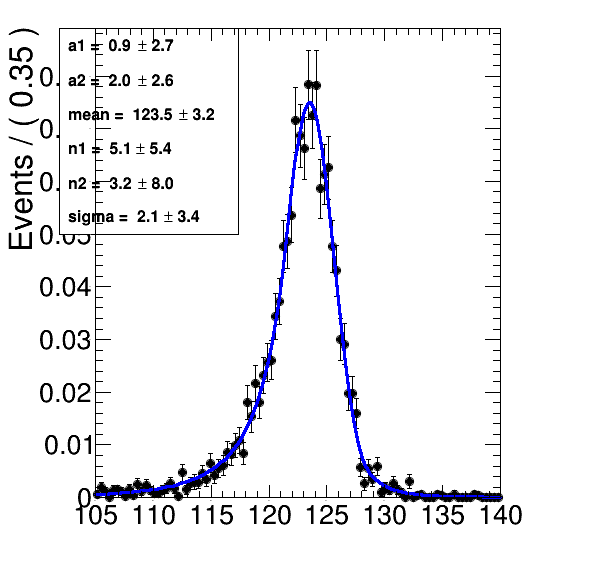
\includegraphics[width=0.32\linewidth]{../AN-18-340/Figures/Signal/fit_stage_ggH_0j_0_10_4e2018.png} % ZHfitM125__4e_UntaggedMor18}
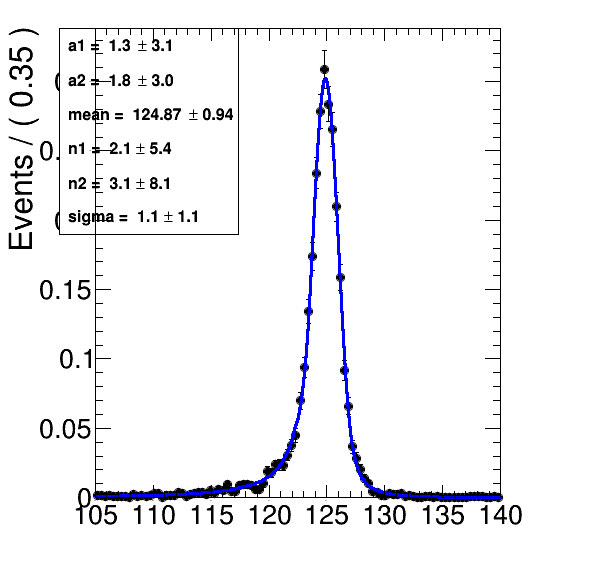
\includegraphics[width=0.32\linewidth]{../AN-18-340/Figures/Signal/fit_stage_ggH_0j_0_10_4mu2018.png} %ZHfitM125__4mu_UntaggedMor18}
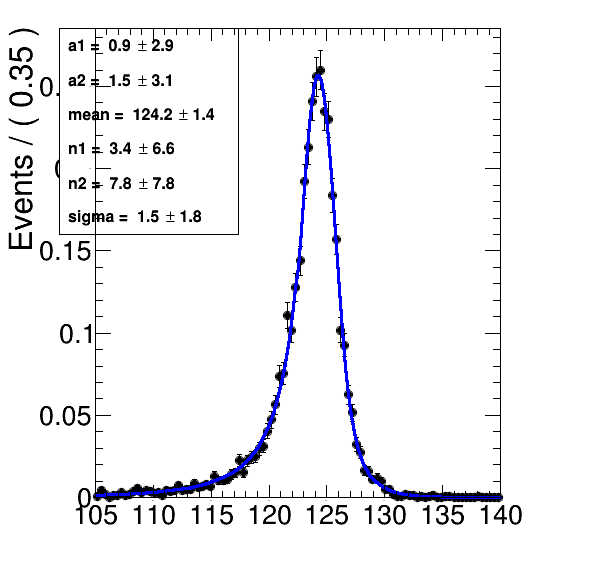
\includegraphics[width=0.32\linewidth]{../AN-18-340/Figures/Signal/fit_stage_ggH_0j_0_10_2e2mu2018.png} %ZHfitM125__2e2mu_UntaggedMor18} \\ %fitM125_ggH_4e_UntaggedMor18.png} %fitM125_ggH_2e2mu_UntaggedMor18.png} \\
\caption{Probability density functions $f(m_{4l}|m_{H})$ for signal
  with {\bf $m_H$=125 \GeV} at the reconstruction level after the full lepton and event selections are applied. The distributions obtained {\bf from 13\TeV} ggH  MC samples are fitted with the model described in the text for  $4\mu$ (left), $4e$ (center) and $2e2\mu$ (right) events. The distribution show the events for $\pt$ below 10 GeV.
\label{fig:sigShapeFits13TeV125}}
\end{figure}



\begin{figure}[!h]
\centering
%
\includegraphics[width=0.32\linewidth]{Figures/Signal/simFit_VBF_2j_mjj_GT700_2j_120_4mu_2018.png} %fitM120_MOR17_ZH_2e2mu_Untagged.pdf}
\includegraphics[width=0.32\linewidth]{../AN-18-340/Figures/Signal/simFit_ggH_0j_0_10_120_2e2mu_2018.png} %fitM120_MOR17_ZH_2e2mu_Untagged.pdf}
\includegraphics[width=0.32\linewidth]{../AN-18-340/Figures/Signal/simFit_ggH_0j_0_10_125_2e2mu_2018.png} %fitM120_MOR17_ZH_2e2mu_Untagged.pdf}
\includegraphics[width=0.32\linewidth]{../AN-18-340/Figures/Signal/simFit_ggH_0j_0_10_130_2e2mu_2018.png} %fitM120_MOR17_ZH_2e2mu_Untagged.pdf}
\caption{Simultaneous fits for  $f(m_{4l}|m_{H})$ for $\ggH$ signal for \pt below 10 GeV
  with {\bf $m_H$=120,125,130 \GeV} at the reconstruction level after the full lepton and event
  selections are applied. The distributions obtained {\bf from 13\TeV}
  $\ggH$ MC samples are fitted with the model described in the text for
  $2e2\mu$  events.
\label{fig:simFitggH}}
\end{figure}







%
%
%
%
%
%
%
%
%
%
%
%
%
%
%
%
%
%
%
%The purpose is to extract integrated and differential fiducial cross sections after corrections of detector effects, resolution and systematic biases. To
%achieve
%this target, the corrections are extracted by using simulated samples and then encoded in the parametrization of $m_{4\ell}$ spectra at the 
%reconstruction level. Then we directly extract the parameter of interest ($\sigma{}_{fid}$) by performing the maximum likelihood fit of background and 
%signal
%parametrization to the observed $m_{4\ell}$ distribution. 
%All the systematic uncertainties in the measurements are encoded as nuisance parameters, which are profited properly in fit procedure. In order to obtain results, we used asymptotic approach~\cite{Cowan:2010js} with test statistics that is based on profile likelihood ratio~\cite{LHC-HCG}. Maximization of  likelihood is performed by fitting simultaneously, in each bin, the signal cross section at the fiducial level with all reconstruction bins and all three final states. 
%The procedure applied for $\Hllll$ fiducial (integrated and differential) cross section measurements will be given in  Sections \ref{sec:SignalInclusive} and \ref{sec:SignalDifferential}. 
%Finally, the unfolding procedure to extract fiducial cross section kinematic observables' bins at the fiducial level, corrected for the detection 
%efficiency and resolution effects, is performed as discussed in Ref.~\cite{Prosper:2011zz} and similar to what is adopted for $H \rightarrow \gamma\gamma$ decay
%channel~\cite{CMS:HIG-14-016}.
%\par 
%Double Crystal Ball function is used for shape description of signal resonant contribution ($\mathcal{P}_{\mathrm{res}}(m_{4\ell})$) ~\cite{Chatrchyan:2013mxa} as is given below, with the yield proportional to the
%parameter of interest ($\sigma_{\mathrm{fid}}$). 
%\begin{equation}\label{eq:dCBDef}
%f_{dCB}(x;\alpha,n,s,\sigma) = N
%\left \{
%    \begin{array}{ll}
%        e^{-\frac{(x-s)^{2}}{2\sigma^2}}  & \mbox{if } -\alpha_{L} < \frac{x-s}{\sigma} < \alpha_{R}  \\
%        A_{L}(B_{L} - \frac{x-s}{\sigma}^{-n_{L}})   & \mbox{if } \frac{x-s}{\sigma} \leq -\alpha_{L} \\
%        A_{R}(B_{R} + \frac{x-s}{\sigma}^{-n_{R}})   & \mbox{if } \frac{x-s}{\sigma} \geq \alpha_{R}
%    \end{array}
%\right \}
%\end{equation}
%
%\begin{center}
%$A_{L} = (\frac{n_{L}}{\alpha})^{n_{L}} \times e^{-\frac{|\alpha_{L}|^{2}}{2}}$
%\end{center}
%
%\begin{center}
%$A_{R} = (\frac{n_{R}}{\alpha})^{n_{R}} \times e^{-\frac{|\alpha_{R}|^{2}}{2}}$
%\end{center}
%
%\begin{center}
%$B_{L} = \frac{n}{\alpha_{L}} - |\alpha_{L}|$
%\end{center}
%
%\begin{center}
%$B_{R} = \frac{n}{\alpha_{R}} - |\alpha_{R}|$
%\end{center}
%
%\begin{center}
%$N$ is the normalization constant.
%\end{center}
%
%
%
%
%\par
%In case of $\W(Z)H$, %$\ZH$ 
%and $t\bar{t}{\rm H}$ modes of Higgs production, the event selection procedure will occasionally select $4\ell$ candidates where minimum one lepton is produced from associated W or Z bosons or jets, and not from $\Hllll$ process.
%Fraction of such signal events in $105 \GeV < \mathrm{m}(4\ell) < 140 \GeV$ mass range mounts to about 4\%, 18\% and 22\% for $\WH$, $\ZH$ and $t\bar{t}{\rm H}$ modes of production, respectively. These events have a broad invariant $m_{4\ell}$ mass distribution
%that depends on the exact production mechanism. The shape of the contribution by this background , $\mathcal{P}_{\mathrm{comb}}(m_{4\ell})$, is described
%a Landau distribution with parameters extracted from simulations. 
%\par 
%$f_{\mathrm{nonfid}}$ represents the ratio of the events reconstructed from out of fiducial region to those reconstructed from within fiducial volume.
%For a particular bin j at reconstruction level, it is given as:
%%The $f_{\mathrm{nonfid}}$ fraction describes the ratio of the nonfiducial and fiducial signal contribution in bin j at the reconstruction level.
%\begin{eqnarray}
%f^{j}_{\mathrm{nonfid}} = \frac{N(\mathrm{j_{reco}} ~\&\&~ \mathrm{not~fid.})}{N(\mathrm{j_{reco}} ~\&\&~ \mathrm{fid.})}.
%\end{eqnarray}
%Such events arise from imperfect detector resolution which causes the differences for quantities calculated at generated and reconstructed levels.
%%such as lepton isolation and other quantities used for the event selection. 
%Fraction of these events are also treated as background and will be referred 
%"non-fiducial signal`` throughout  this disseration. It has been demonstrated with MC samples that these events can be described using same shape as resonant
%component. The values of such fraction are extracted from simulation repeatedly for SM. This fraction varies among different production modes of Higgs e.g. it is  4\%  for the $\ggH$ and 3\% for $ttH$ production mode. The values for each model are listed in the Tables \ref{tab:summarySM2016},  \ref{tab:summarySM2017} and  \ref{tab:summarySM2018} for 2016, 2017 and 2018 respectively. %Tables~\ref{tab:Accept_Eff_fOut}, \ref{tab:Accept_Eff_fOut_7TeV} for 
%%8 and 7~TeV respectively.
%\par  
%To make comparison with the  theoretical predictions, measurements need corrections for resolution of detector and effects of efficiency. To unfold 
%reconstruction-level distribution to the distribution before all detector effects, the efficiency matrix ($\epsilon$) is constructed using the signal
%MC samples. The efficiency matrix ($\epsilon$) provides the probability of an event that was generated in $i$th bin at the fiducial level and is reconstructed 
%in j-th bin as:
%\begin{equation}
%\epsilon_{i,j} = \frac{N(\mathrm{j_{reco}} ~\&\&~ \mathrm{i_{gen}})}{N(\mathrm{i_{gen}})}\ ,
%\end{equation}
%where $N(i_{gen})$ is total number of the events in $i$th bin at fiducial level and $N(\mathrm{j_{reco}} ~\&\&~ \mathrm{i_{gen}})$ is total number events which $i$th bin at the fiducial level but reconstructed in $j$th bin. For integrated measurements, where we have only one bin, fiducial efficiency is 
%about 65\% which can change upto 7\% for other signal models. For differential measurements, it is described by detector response matrix for each observable.
%Figure \ref{fig:eff-pT4l-4e} shows the efficiency matrix for $p_{T}(H)$  measurement using different SM production MC samples. The efficiency matrix is
%dominated by diagonal elements, but in general it can have non-negligible off-diagonal elements specially for jet related observables due to
%jet energy scale uncertainty. In case of differential variable, jet multiplicity,  neighbour elements of diagonal varies from 3\% to 21\% as shown in Figures
%\ref{fig:eff-njets_reco_pt30_eta4p7-4e}-\ref{fig:eff-njets_reco_pt30_eta4p7-2e2mu} in the Appendix \ref{app:siginputs}.
%\par The estimated number events for a studied differential observable in a final state $f$ and in the defined bin $i$ are described in terms of $m_{4\ell}$ given by:
%\begin{eqnarray}
%\label{eqn:m4l}
%\begin{aligned}
%N_{\mathrm{obs}}^{\mathrm{f},i}(m_{4\ell}) &= N_{\mathrm{fid}}^{\mathrm{f},i}(m_{4\ell})+N_{\mathrm{nonfid}}^{\mathrm{f},i}(m_{4\ell})+N_{\mathrm{comb}}^{\mathrm{f},i}(m_{4\ell})+N_{\mathrm{bkg}}^{\mathrm{f},i}(m_{4\ell}) \\
%&=\sum_{j} \epsilon_{i,j}^{\mathrm{f}} \cdot \left(1+f_{\rm nonfid}^{\mathrm{f},i} \right)\cdot\sigma_{\mathrm{fid}}^{\mathrm{f},j} \cdot \mathcal{L}\cdot\mathcal{P}_{\mathrm{res}}(m_{4\ell}) \\
%&~~~~~+ N_{\mathrm{comb}}^{\mathrm{f},i}\cdot\mathcal{P}_{\mathrm{comb}}(m_{4\ell})+N_{\mathrm{bkg}}^{\mathrm{f},i}\cdot\mathcal{P}_{\mathrm{bkg}}(m_{4\ell}).
%\end{aligned}
%\end{eqnarray}
%Where  $N_{\mathrm{fid}}^{\mathrm{f},i}(m_{4\ell})$, $N_{\mathrm{nonfid}}^{\mathrm{f},i}(m_{4\ell})$, $N_{\mathrm{comb}}^{\mathrm{f},i}(m_{4\ell})$
%and $N_{\mathrm{bkg}}^{\mathrm{f},i}(m_{4\ell})$ denote the resonant fiducial signal, the nonfiducial resonant, the combinatorial contribution of
%fiducial signal, and background contributions in a defined bin $i$ as functions of $m_{4\ell}$ (four lepton invariant mass), respectively.
%Then, probability density functions corresponding to the resonant (fiducial and the nonfiducial) signal, the combinatorial contributions of fiducial signal, and contribution from the background  are  $\mathcal{P}_{\mathrm{res}}(m_{4\ell})$, $\mathcal{P}_{\mathrm{comb}}(m_{4\ell})$ and $\mathcal{P}_{\mathrm{bkg}}(m_{4\ell})$  respectively.
% $\epsilon_{i,j}^{\mathrm{f}}$ is  the  response matrix that connects reconstructed level events in a defined bin $i$ with fiducial events in the bin $j$
%for studied differential observable. The $f_{\rm nonfid}^{i}$ fraction represents the ratio of nonfiducial signal to the fiducial signal contributions 
%in a defined bin $i$ at reconstruction level. $\sigma_{\mathrm{fid}}^{\mathrm{f},j}$ is the parameter of interest that represents signal cross section for a final
%state f in a defined bin $j$ of fiducial region.
%
